\begin{exercício}{Condições de contorno da Eletrostática em meios materiais}{exercício1}
    Faça um resumo das condições de contorno da Eletrostática em meios materiais, em termos dos campos \(\vetor{E}, \vetor{D}\) e \(\vetor{P}\).
\end{exercício}
\begin{proof}[Resolução]
    Consideremos uma superfície \(\Sigma\) de interface entre dois abertos \(\Omega_1\) e \(\Omega_2\), nos quais os campos elétricos \(\vetor{E}_1\) e \(\vetor{E}_2\) estão definidos.
    \begin{center}
        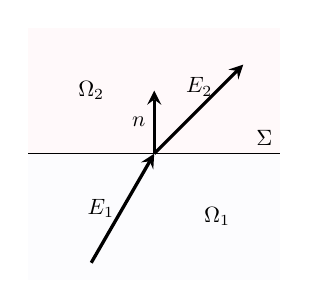
\begin{tikzpicture}[scale = 0.8, every node/.style={scale = 0.8}]
            \fill[Lavender!10] (-2,-2) rectangle (2,0);
            \fill[Pink!10] (-2,0) rectangle (2,2);
            \draw[-] (-2,0) -- (2,0) node[left, anchor = south east] {\(\Sigma\)};

            \draw[very thick, -stealth] (0,0) -- +(90:1) node[midway, left] {\(\vetor{n}\)};
            \draw[very thick, -stealth] (0,0) -- +(45:2) node[near end,left] {\(\vetor{E}_2\)};
            \draw[very thick, stealth-] (0,0) -- +(-120:2) node[midway,left] {\(\vetor{E}_1\)};

            \node at (-1,1) {\(\Omega_2\)};
            \node at (1,-1) {\(\Omega_1\)};
        \end{tikzpicture}
    \end{center}
    Seja \(\vetor{n}\) o vetor normal de \(\Sigma\), orientado no sentido de \(\Omega_1\) a \(\Omega_2\). Sendo \(\sigma\) a distribuição superficial de cargas em \(\Sigma\), segue pela lei de Gauss que
    para todo ponto de \(\Sigma\).

    Consideremos um volume cilíndrico \(V\) centrado em um ponto de interesse na superfície \(\vetor{\x} \in \Sigma\) de altura \(2h\), de área transversal \(\delta S\), e coaxial com o vetor normal em \(\vetor{n}(\vetor{\x})\). Sendo \(S_L\) a superfície lateral de \(\partial V\), e \(S_i = \Omega_i \cap (\partial V \setminus S_L)\), temos
    \begin{equation*}
        \int_{V \cap \Omega_1} \dln3{\x'}\frac{\rho_1(\vetor{\x'})}{\epsilon_0} + \int_{V\cap \Omega_2} \dln3{\x'}\frac{\rho_2(\vetor{\x'})}{\epsilon_0}+ \int_{V\cap \Sigma} \dln2{\x'}\frac{\sigma(\vetor{\x'})}{\epsilon_0} = \int_{S_L} \dln2{\x'} \inner{\vetor{n'}}{\vetor{E}(\vetor{\x'})} + \sum_{i=1}^2 \int_{S_i} \dln2{\x'} \inner{\vetor{n'}}{\vetor{E}_i(\vetor{\x'})}
    \end{equation*}
    pela lei de Gauss. Tomando o limite em que \(h \to 0\) e considerando \(\delta S\) suficientemente pequeno, temos
    \begin{equation*}
        \frac{\sigma(\vetor{\x})}{\epsilon_0}\delta S \simeq \inner{\vetor{n}}{\vetor{E}_2(\vetor{\x})} \delta S - \inner{\vetor{n}}{\vetor{E}_1(\vetor{\x})} \delta S
    \end{equation*}
    donde segue que
    \begin{equation*}
        \inner*{\vetor{n}(\vetor{\x})}{\vetor{E}_2(\vetor{\x}) - \vetor{E}_1(\vetor{\x})} = \frac{\sigma(\vetor{\x})}{\epsilon_0},
    \end{equation*}
    para todo \(\vetor{\x} \in \Sigma\).

    Seja \(\vetor{v} \in T\Sigma\) um vetor normalizado do espaço tangente de \(\Sigma\), então \(\set{\vetor{v}, \vetor{n}\times\vetor{v}, \vetor{n}}\) é uma base ortonormal positivamente orientada de \(\mathbb{R}^3\). Consideremos uma superfície \(\Pi\) retangular de altura \(2h\) paralelo a \(\vetor{n}(\vetor{\x})\), de largura \(\delta L\) paralela a \(\vetor{n}(\vetor{\x}) \times \vetor{v}(\vetor{\x})\), e centrado em \(\vetor{\x} \in \Sigma\). No limite em que \(h \to 0\) temos
    \begin{equation*}
        0 = \oint_{\partial\Pi} \dl{\vetor{\ell}}\cdot{\vetor{E}} = \inner{\vetor{n}(\vetor{\x})\times\vetor{v}(\vetor{\x})}{\vetor{E}_1(\vetor{\x}) - \vetor{E}_2(\vetor{\x})}\delta L \implies \inner*{\vetor{v}(\vetor{\x})}{\left[\vetor{E}_1(\vetor{\x}) - \vetor{E}_2(\vetor{\x})\right]\times \vetor{n}(\vetor{\x})} = 0.
    \end{equation*}
    Como \(\vetor{v}\) é arbitrário, obtemos
    \begin{equation*}
        \left[\vetor{E}_1(\vetor{\x}) - \vetor{E}_2(\vetor{\x})\right]\times \vetor{n}(\vetor{\x}) = 0
    \end{equation*}
    para todo \(\vetor{\x} \in \Sigma\).

    Pelos mesmos argumentos, e utilizando as relações
    \begin{equation*}
        \nabla \cdot \vetor{D} = \rho_l, \quad
        \nabla \cdot \vetor{P} = \rho_p,\quad
        \nabla\times \vetor{D} = \nabla\times \vetor{P},
    \end{equation*}
    temos
    \begin{equation*}
        \inner*{\vetor{n}(\vetor{\x})}{\vetor{D}_2(\vetor{\x}) - \vetor{D}_1(\vetor{\x})} = \sigma_l(\vetor{\x}),
    \end{equation*}
    \begin{equation*}
        \inner*{\vetor{n}(\vetor{\x})}{\vetor{P}_2(\vetor{\x}) - \vetor{P}_1(\vetor{\x})} = \sigma_p(\vetor{\x}),
    \end{equation*}
    e
    \begin{equation*}
        \left\{\left[\vetor{D}_1(\vetor{\x}) - \vetor{P}_1(\vetor{\x})\right] - \left[\vetor{D}_2(\vetor{\x}) - \vetor{P}_2(\vetor{\x})\right]\right\}\times \vetor{n}(\vetor{\x}) = 0
    \end{equation*}
    para todo \(\vetor{\x} \in \Sigma\). Desse modo, para meios lineares, temos
    \begin{equation*}
        \inner*{\vetor{n}(\vetor{\x})}{\epsilon_2\vetor{E}_2(\vetor{\x}) - \epsilon_1\vetor{E}_1(\vetor{\x})} = \sigma_l(\vetor{\x}),
    \end{equation*}
    onde \(\epsilon_i = (1 + \chi_i)\epsilon_0\).
\end{proof}
